\chapter{Ispitivanje}
Tijekom ispitivanja korišten je USB ispitivač UT658DUAL tvrtke Changan UNI-T prikazan na slici \ref{slk:UT658DUAL}. Ovaj uređaj se može spojiti između USB izvora i uređaja te pokazuje razinu napona, jakost struje koju izvor daje, količinu potrošenog naboja u mAH i vrijeme trajanja mjerenja.
\begin{figure}[htb]
    \centering
    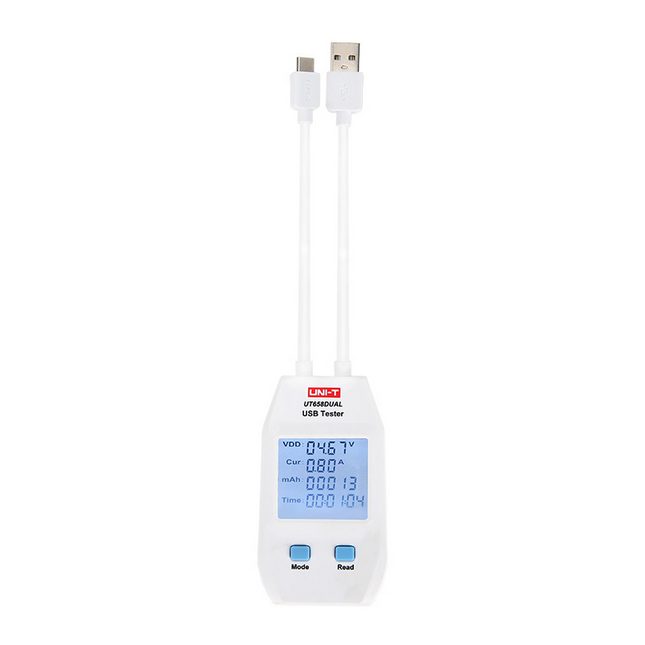
\includegraphics[width=6 cm]{Figures/UT658DUAL.png}
    \caption{USB ispitivač UT658DUAL}
    \label{slk:UT658DUAL}
\end{figure}
\section{Središnji uređaj}
Na slikama \ref{slk:MB_TEST_01} i \ref{slk:MB_TEST_02} prikazano je ispitivanje središnjeg uređaja. Umjesto priključka za bateriju namontiran je držač za standardnu 18650 bateriju radi lakšeg testiranja. Naime, baterija se često vadi i stavlja tijekom testiranja, a odabran priključak je predviđen da se rijetko otkapča, pa ga je radi toga i teško otkopčati.
\begin{figure}[htb]
    \centering
    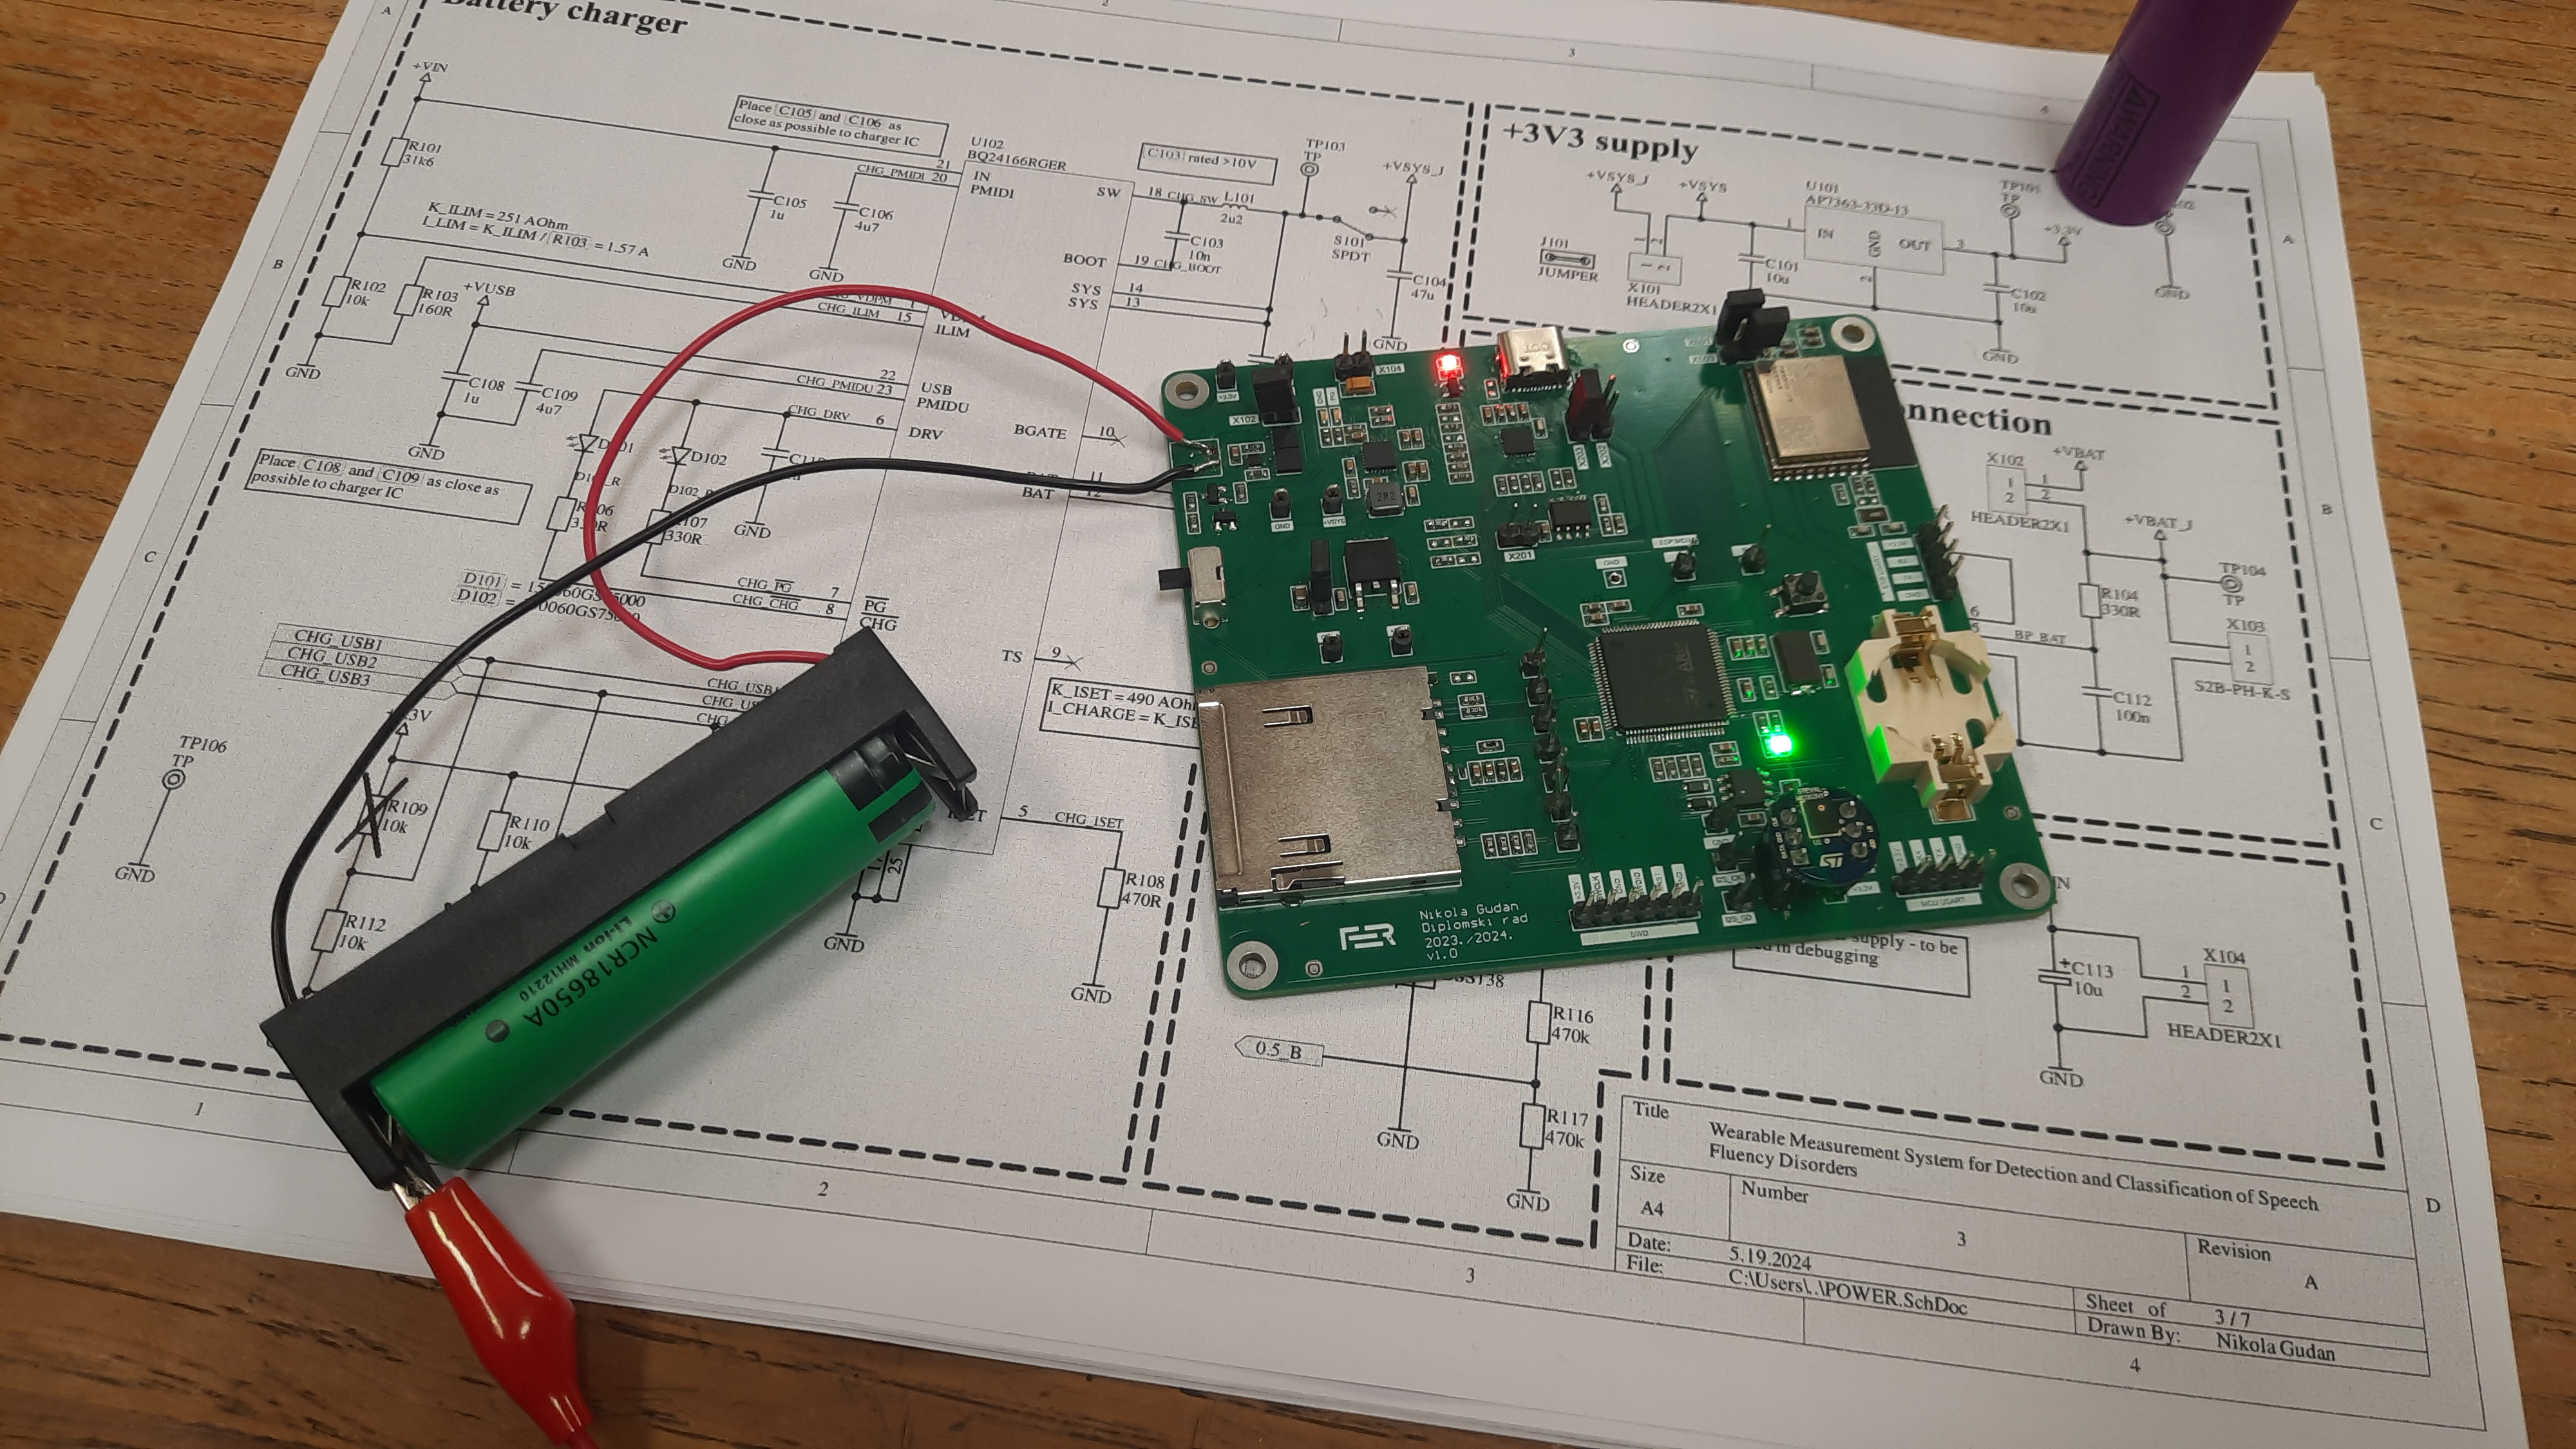
\includegraphics[width=10 cm]{Figures/MB_TEST_01.jpg}
    \caption{Ispitivanje pločice središnjeg uređaja}
    \label{slk:MB_TEST_01}
\end{figure}
\begin{figure}[htb]
    \centering
    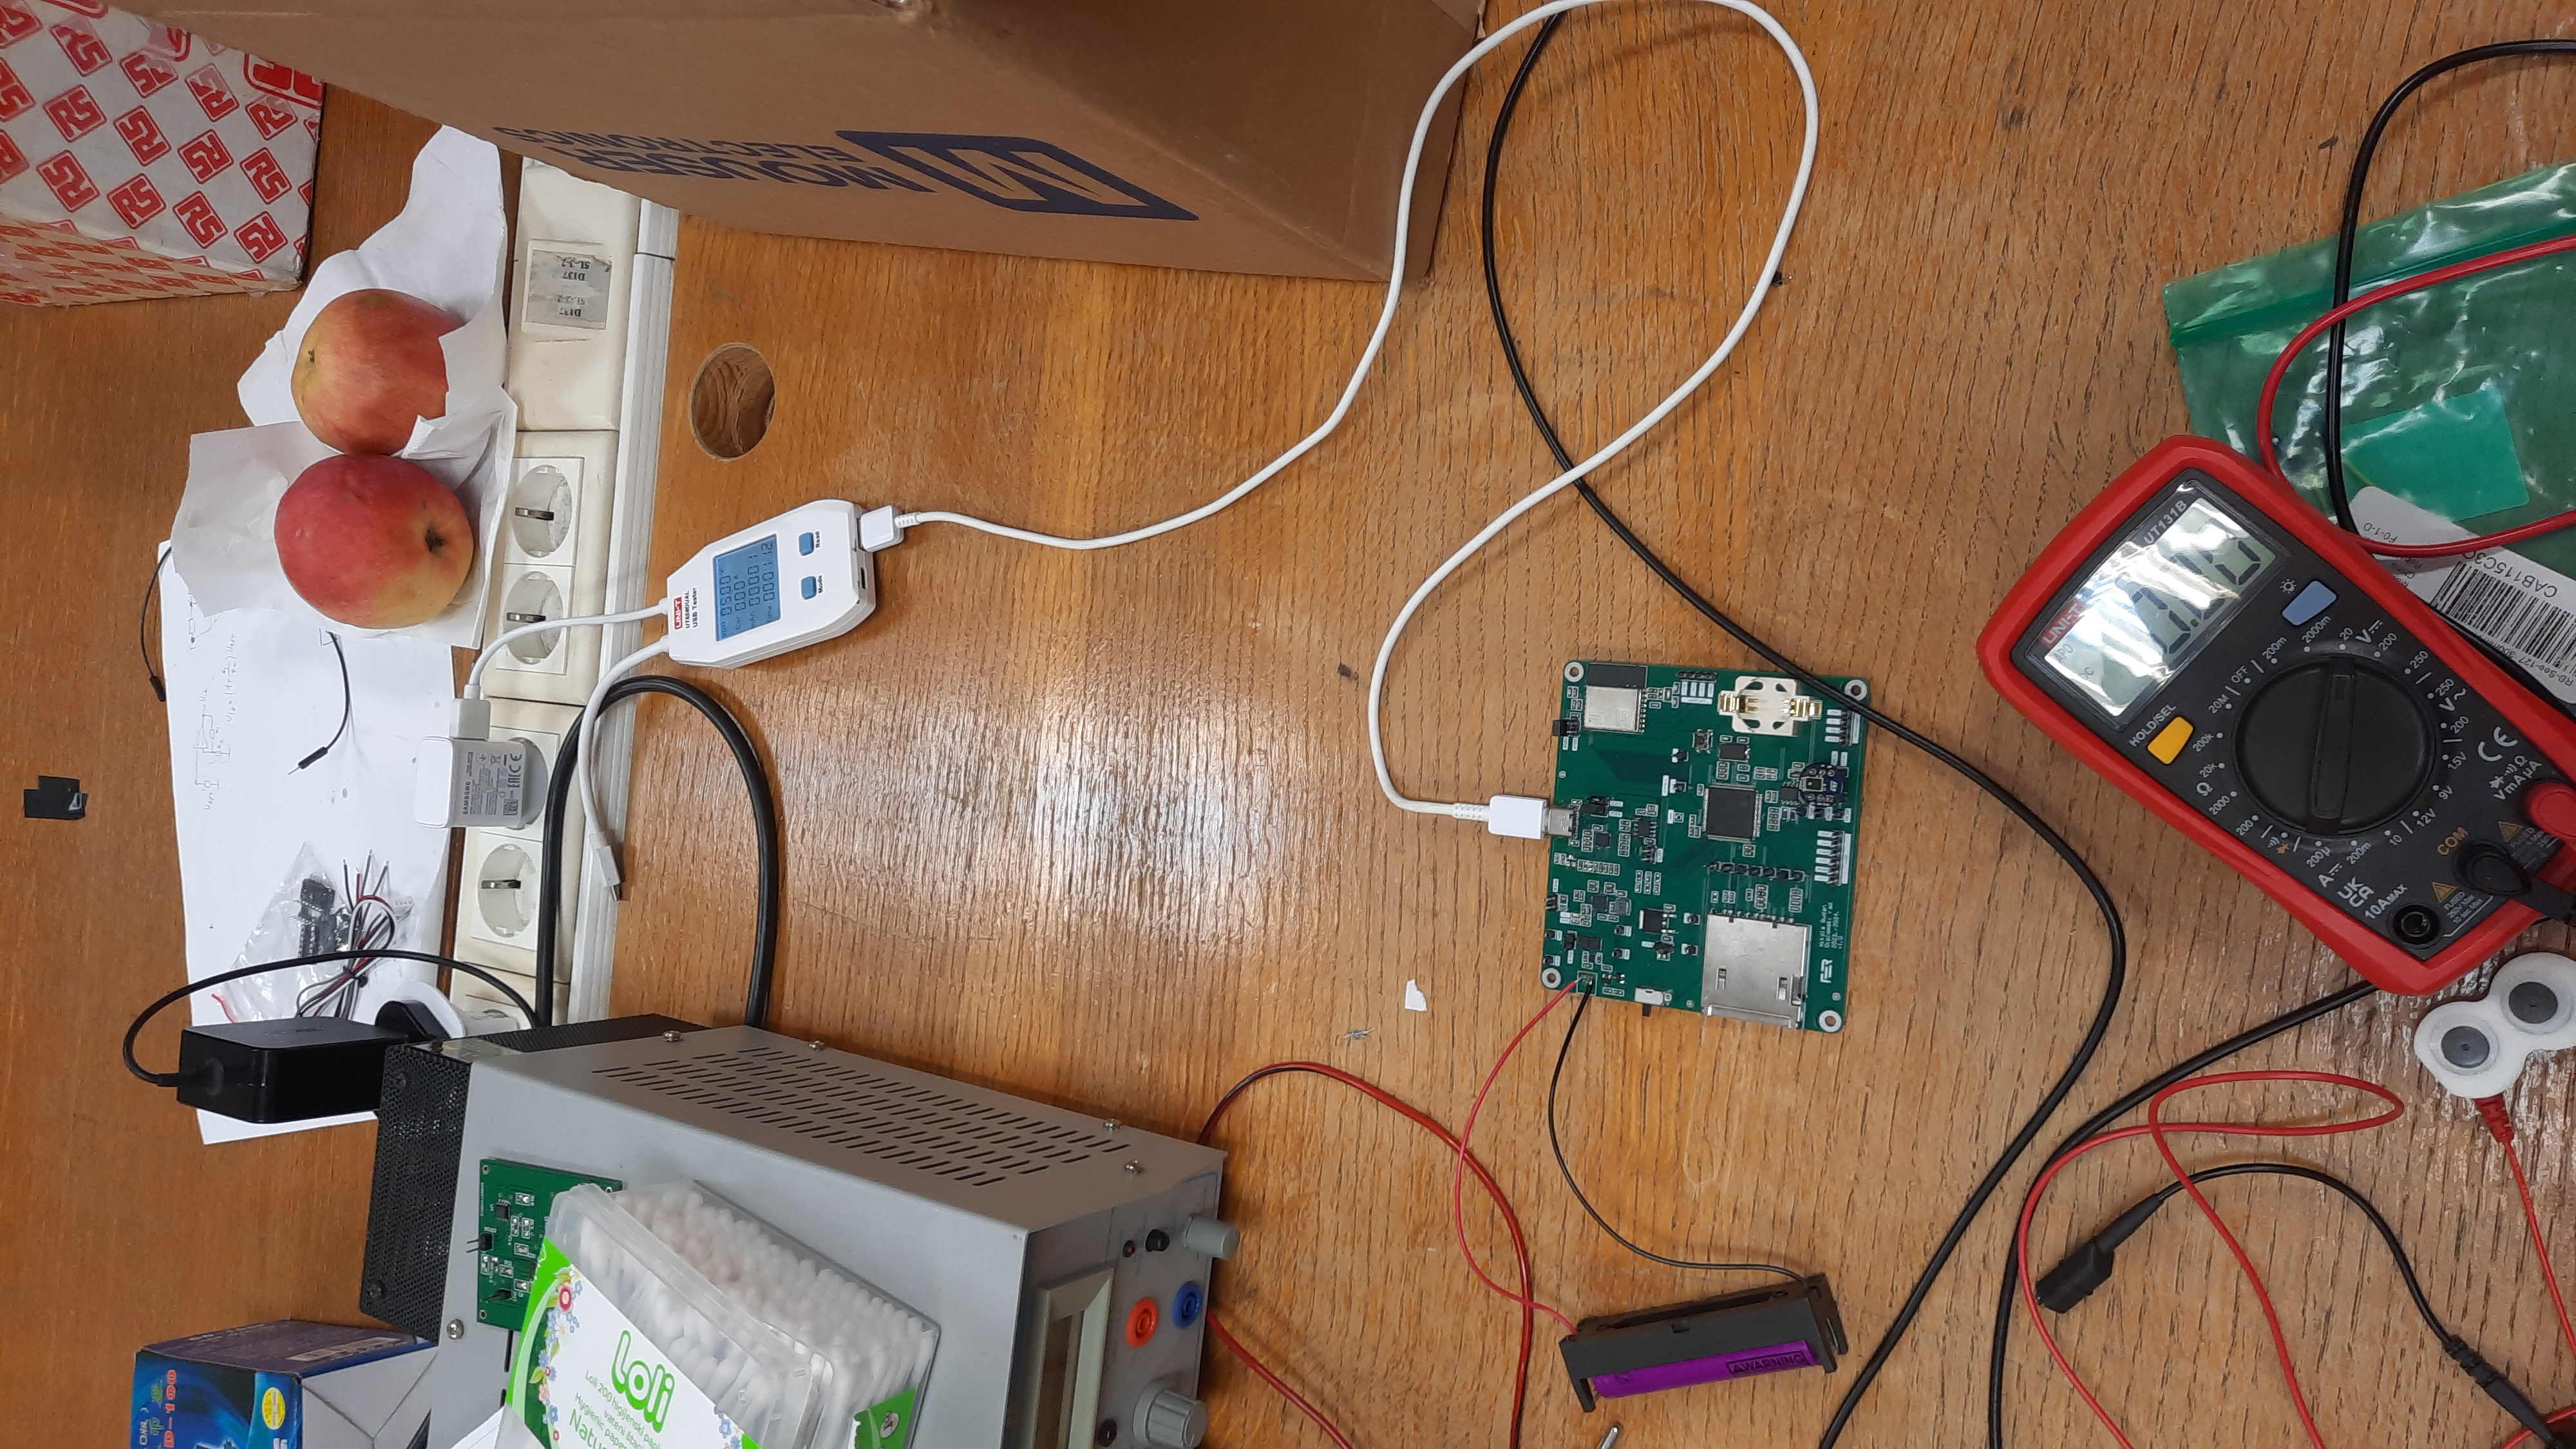
\includegraphics[width=10 cm]{Figures/MB_TEST_02.jpg}
    \caption{Postava ispitivanja pločice središnjeg uređaja}
    \label{slk:MB_TEST_02}
\end{figure}

Oktrivena je greška u dizajnu USB napajanja. Kada se ukopča USB, bez obzira na to da li izvor podržava zatraženu snagu ili ne, napajanje sa USB-a se ne prosljeđuje dalje na ostatak sustava. Problem se nalazi u tranzistorskoj sklopci (slika \ref{slk:MB_USB}). Naime, kada čip pokuša uključiti tranzistore, na prvom tranzistoru dolazi do pada napona na porednoj diodi koja se nalazi unutar tranzistora, pa se na uvodu drugog tranzistora nalazi napon napajanja umanjen za napon provoda diode (između 0.5 V i 1.2 V \cite{di:dmp3098}). Čip je preko VDC\_OUT stezaljke onda detektirao prevelik pad napona i onemogućio napajanje sa USB-a. Radi toga su napravljene izmjene u USB napajanju kod narukvice vidljive na slici \ref{slk:BR_USB}.

Kada baterija nije bila ukopčana, nije bilo moguće uključiti USB napajanje iz razloga objašnjenog u potpoglavlju \ref{sec:BR_USB}. Ukratko, čip nije mogao postaviti odgovarajuće otpornike na CC linije pa se nije mogla zatražiti nikakva snaga od USB izvora.

Tijekom testiranja punjača utvrđeno je da punjač može bez problema proslijediti napon baterije na izlaz. Međutim, kada se je priključio vanjski napon, bilo na USB ili preko priključka za laboratorijski izvor napona u svrhu punjenja baterije, punjač više nije radio. Bilo je vidljivo trepteranje svjetlećih dioda za indikaciju ispravnog napajanja i punjenja u frekvenciji 1 treptaj po sekundi. Naime, dolazi do aktiviranja temperaturne zaštite na način opisan u potpoglavlju \ref{sec:BR_BATCHG}.

Tijekom čekanja izrade tiskane pločice, razvijena je cjelokupna programska podrška za središnji uređaj. S obzirom na to da većina napajanja, izuzev baterije, nije radila, tijekom testiranja programske podrške, a samim time i digitalnog dijel sustava, uređaj se je napajao preko programatora, koji je bio priključen na pločicu cijelo vrijeme tijekom testiranja programske podrške. Utvrđeno je da mikrofon normalno snima govor, mikrokontroler komunicira sa svim podsustavima te također bez poteškoća obrađuje i sprema podatke na SD karticu, bežični podsustav se uspješno može programirati i RTC mjeri vrijeme napajavši se sa litijske baterije. Dakle, digitalni dio sustava u potpunosti radi.

\section{Narukvica}

Na temelju ispitivanja središnjeg uređaja, napravljene su izmjene i popravci napajanja opisani u poglavlju \ref{pog:bracelet}.
\begin{figure}[htb]
    \centering
    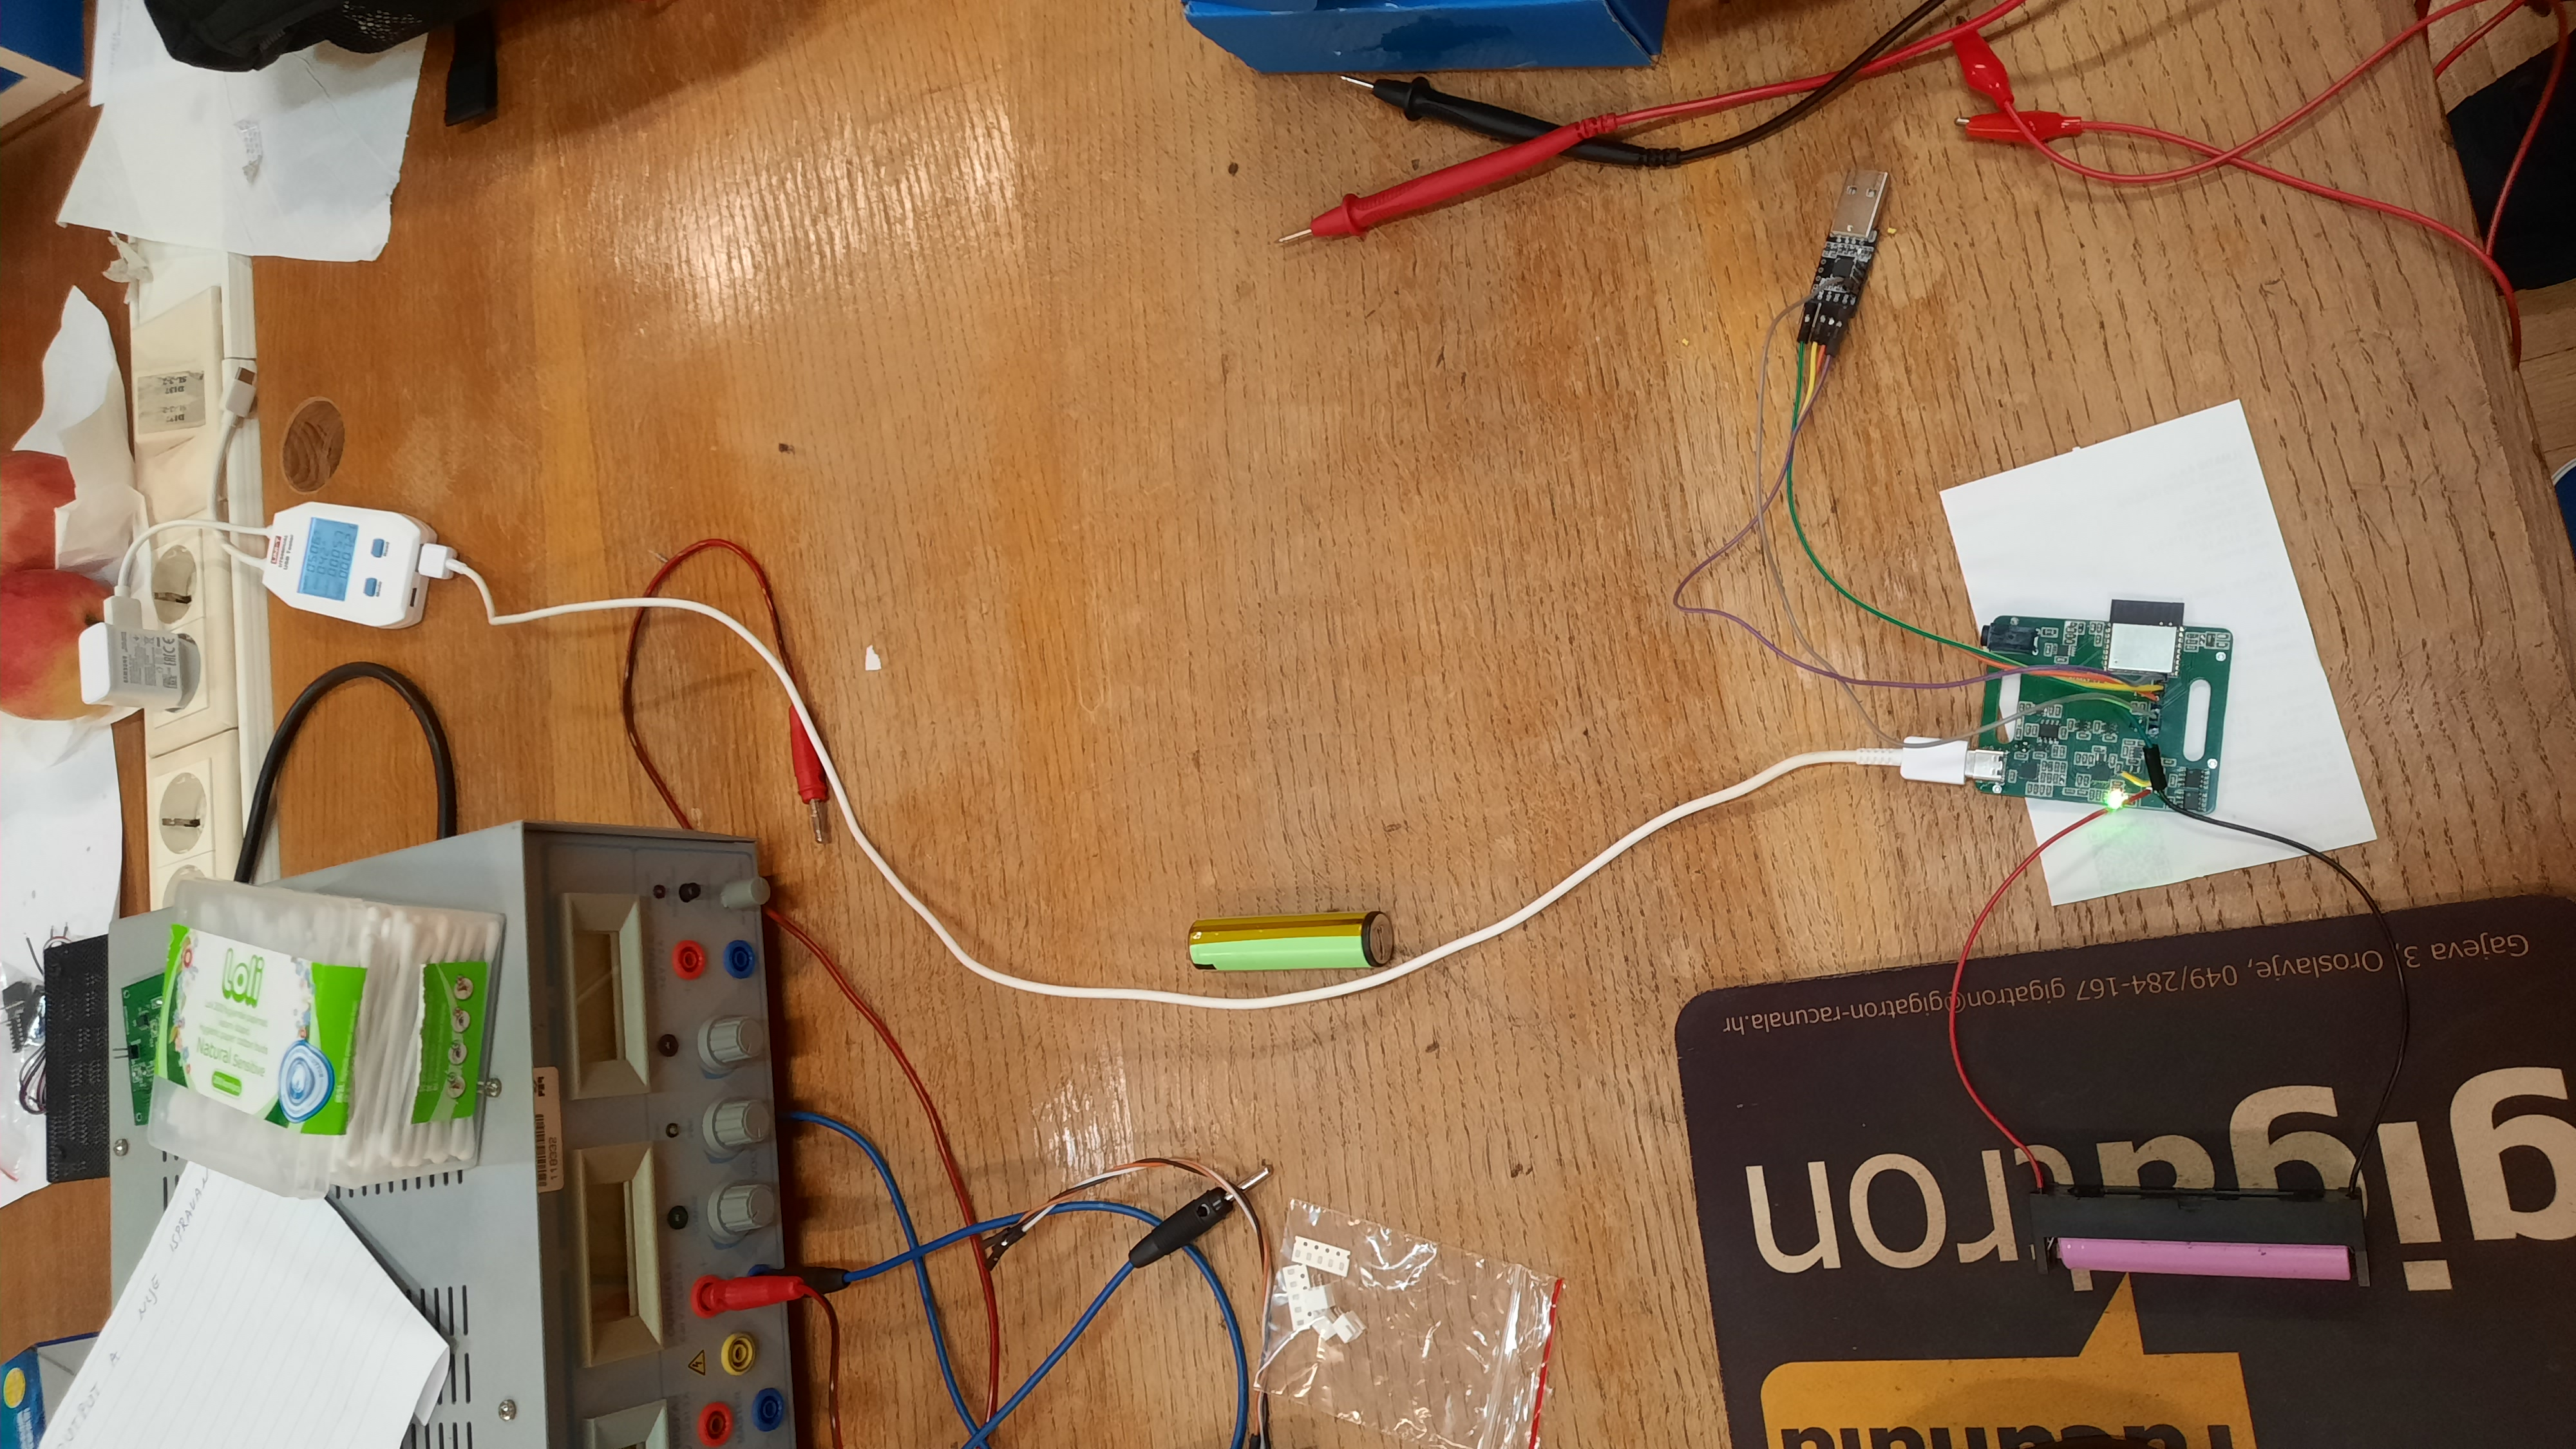
\includegraphics[width=10 cm]{Figures/BR_TEST_02.jpg}
    \caption{Postava ispitivanja pločice narukvice}
    \ref{slk:BR_TEST_01}
\end{figure}